\chapter{Implementation}
\label{ch:implementation}

In this chapter the implementation is discussed, presenting how the objects are detected and how the symbolic predicates are obtained. 

\section{Object detection} 

To interact with the objects we have first to detect them. To do so, they need to be segmented since the algorithm is dealing with unknown objects it is not going to recognize an object as a particular one, instead it segments the objects in the scene. 

This stage is composed of 3 steps:
\begin{enumerate}
\item Filtering the point cloud
\item Detecting the tabletop objects
\item Segmenting the tabletop objects
\end{enumerate}
The Kinect camera is recording a depth image which is quite noisy, overall at the edges, for a proper segmentation is better applying a filter. Fort this we used the statistical outlier removal algorithm \citep{rusu2008towards}.	
Next, since the objects are on a table, the algorithm has to detect first the table, and so the objects that stand on top of it, and then segmenting them. We don't want to segment the entire image, if so, the table would be segmented as an object, and the floor as well.

\subsection{Tabletop Object Detection} 
The strategy for the tabletop object detection phase is composed of 3 different steps:
\begin{enumerate}
\item \textbf{Table plane estimation} (by RANSAC): the points of the table are detected estimating a plane in the point cloud, all the points which belong to such a plane are the points of the table. 
\item \textbf{2D Convex Hull of the table}: having the points of the table a 2D convex hull is computed in order to get a 2D shape containing those points.
\item \textbf{Polygonal prism projection}: all the points are projected on the table plane previously estimated and all the points which projections belong to the 2D convex hull are considered to be points of tabletop objects. The points that do not belong to it are points of non-tabletop objects.
\end{enumerate}

\begin{figure}[tb]
\centering
\begin{subfigure}[t]{0.32\textwidth}
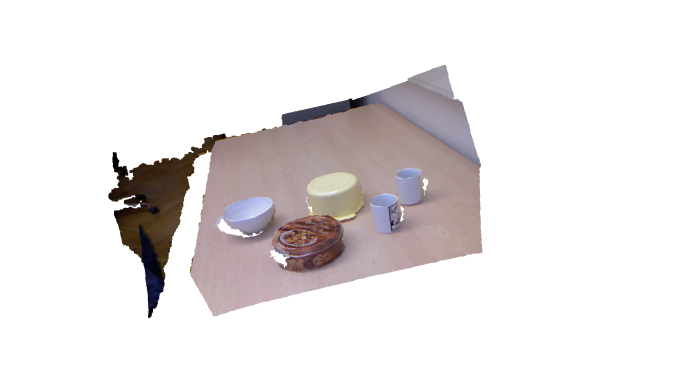
\includegraphics[width = 1.1\textwidth]{Img/ObjectSegmentation/pcl.png}
\caption{Input Point Cloud}\label{img:obj_pointcloud}
\end{subfigure}
\begin{subfigure}[t]{0.32\textwidth}
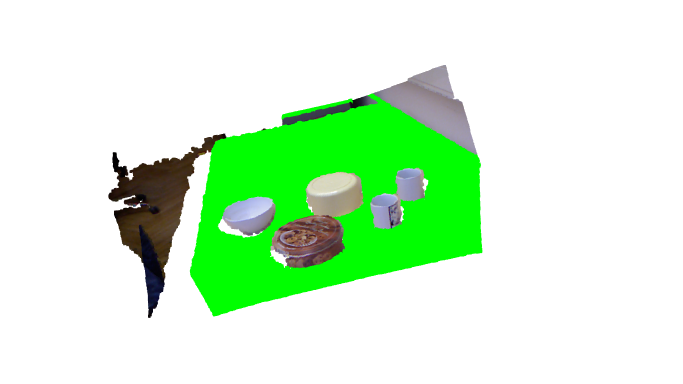
\includegraphics[width = 1.1\textwidth]{Img/ObjectSegmentation/ransac.png}
\caption{RANSAC plane estimation}\label{img:obj_ransac}
\end{subfigure}
\begin{subfigure}[t]{0.32\textwidth}
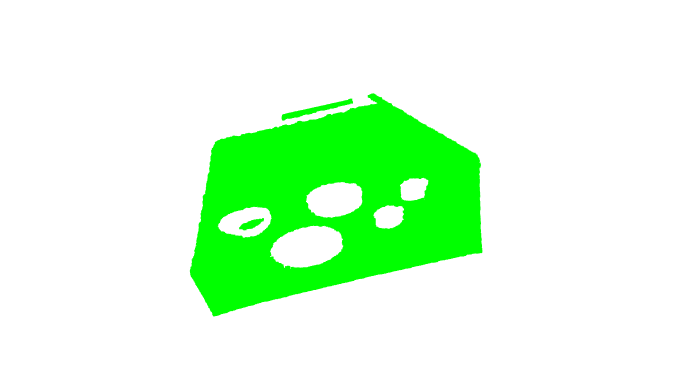
\includegraphics[width = 1.1\textwidth]{Img/ObjectSegmentation/plane.png}
\caption{Table plane}\label{img:obj_plane}
\end{subfigure}
\begin{subfigure}[t]{0.32\textwidth}
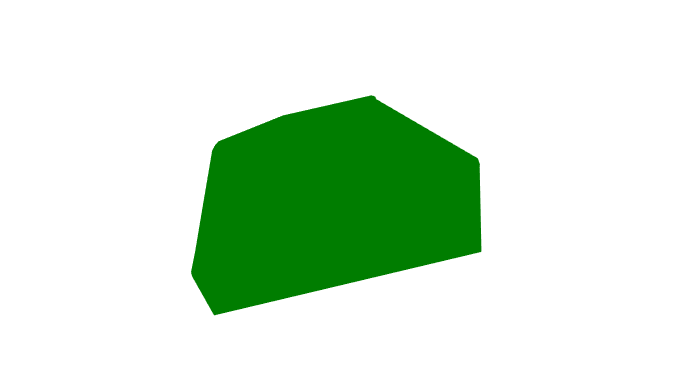
\includegraphics[width = 1.1\textwidth]{Img/ObjectSegmentation/convex_hull.png}
\caption{Convex Hull}\label{img:obj_conex_hull}
\end{subfigure}
\begin{subfigure}[t]{0.32\textwidth}
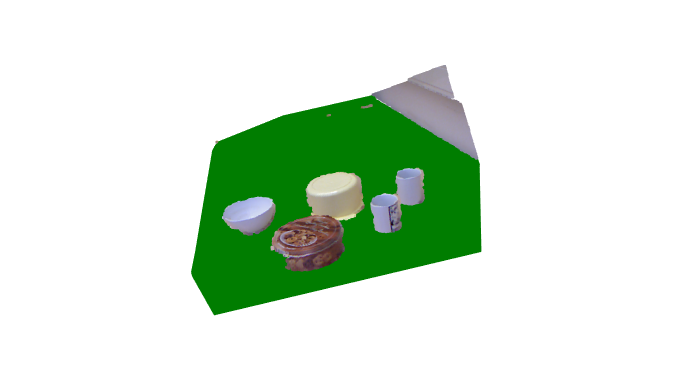
\includegraphics[width = 1.1\textwidth]{Img/ObjectSegmentation/convex_hull_full.png}
\caption{Convex hull in the point cloud}\label{img:obj_convex_hull_full}
\end{subfigure}
\begin{subfigure}[t]{0.32\textwidth}
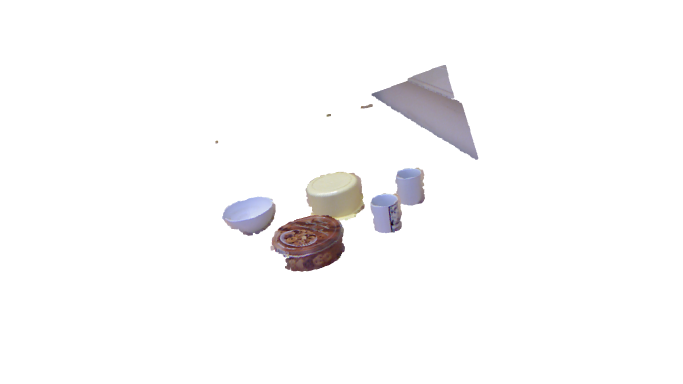
\includegraphics[width = 1.1\textwidth]{Img/ObjectSegmentation/tabletop_objects.png}
\caption{Tabletop objects}\label{img:obj_tabletop_objects_results}
\end{subfigure}
\caption{\textbf{Object Segmentation:} Given the point cloud (\subref{img:obj_pointcloud}), the estimated table's plane is obtained (\subref{img:obj_ransac} and \subref{img:obj_plane}), its convex hull is extracted (\subref{img:obj_conex_hull} and \subref{img:obj_convex_hull_full}), and the tabletop objects are obtained by a polygonal prism projection (\subref{img:obj_tabletop_objects_results}).}
\label{img:obj_tabletop_objects}
\end{figure}

The steps of this tabletop object detection algorithm are described in Figure \ref{img:obj_tabletop_objects}   for the point cloud\footnote{Point cloud taken from the Object Segmentation Database (OSD) \href{http://users.acin.tuwien.ac.at/arichtsfeld/?site=4}{http://users.acin.tuwien.ac.at/arichtsfeld/?site=4}} in Figure \ref{img:obj_pointcloud}.

\subsection{Object Segmentation}
\label{sec:obj_seg}
Once the objects on the table are detected the following phase is to segment them in order to get a point cloud per object.

\subsubsection{Supervoxel}

For their segmentation the supervoxel concept is used. A supervoxel is a group of voxels that share similar characteristics, for instance similar normals.

In this work the supervoxels are computed with the \textit{Voxel Cloud Connectivy Segmentation} (\texttt{VCCS}) algorithm \cite{Papon13CVPR}, which is able to be used in online applications. An example of the obtained supervoxels is shown in Figure \ref{fig:voxels_results}.

The algorithm works in 3 main steps:
\begin{itemize}
\item Voxelizing the point cloud.
\item Creating an adjacency graph for the voxel-cloud.
\item Clustering together all adjacent voxels which share similar features.
\end{itemize} 

\begin{figure}[tb]
\centering
\begin{subfigure}[t]{0.3\textwidth}
\centering
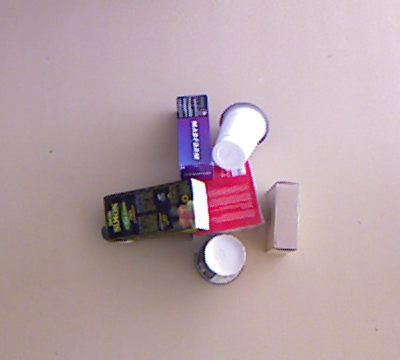
\includegraphics[width=4cm]{Img/ObjectSegmentation/seg1_rgb.png}
\caption{Input scene}
\end{subfigure}
\begin{subfigure}[t]{0.3\textwidth}
\centering
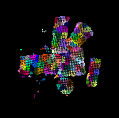
\includegraphics[width=4cm]{Img/ObjectSegmentation/voxel2.png}
\caption{Supervoxels}
\end{subfigure}
\begin{subfigure}[t]{0.3\textwidth}
\centering
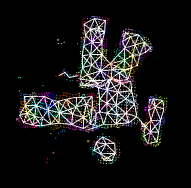
\includegraphics[width=4cm]{Img/ObjectSegmentation/voxel1.png}
\caption{Adjacency graph}
\end{subfigure}
\caption{Example of supervoxels for the table top objects.}\label{fig:voxels_results}
\end{figure}

\subsubsection{Local Convex Connected Patches Segmentation}
\label{sec:LCCP}
Once the supervoxels of the tabletop objects are computed, they can be clustered in order to segment the objects. Papon et al. \citep{LCCP} also proposed a segmentation algorithm based on their supervoxel technique, called \textit{Local Convex Connected Patches Segmentation} (\texttt{LCCP}). This algorithm permits to segment objects by clustering together adjacent convex supervoxels, in Figure \ref{img:LCCP_structure} the algorithm is briefly described.   The algorithm is quite simple but very good for segmentation of objects that have convex shapes. 

\begin{figure}[tb]
\centering
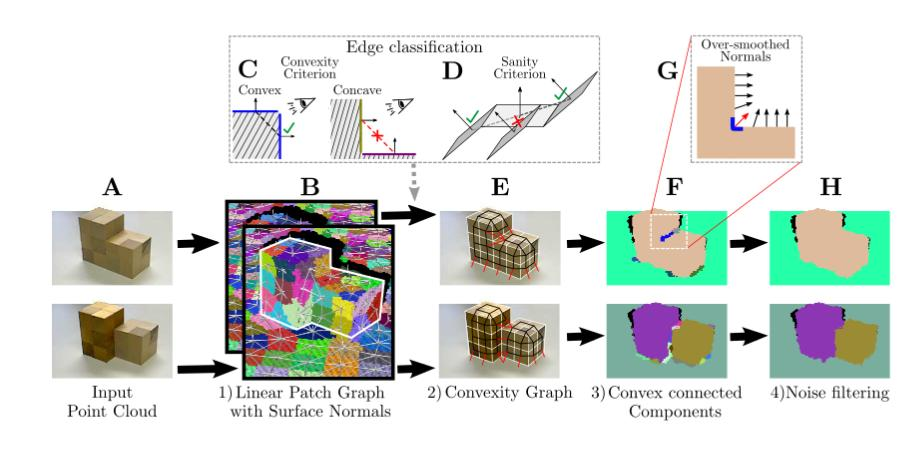
\includegraphics[width=\textwidth]{Img/ObjectSegmentation/lccp_structure.jpg}
\caption{\texttt{LCCP} algorithm's structure. Reproduced from \citep{LCCP}}
\label{img:LCCP_structure}
\end{figure}

It clusters all the adjacent convex supervoxels (patches) using 2 criterion:
\begin{itemize}
\item Extended criterion: to consider two adjacent patches convex, both must have a connection to a patch which is convex with respect both patches
\item Sanity Criterion: check if the adjacent patches which can be considered as convex present geometric discontinuities (see point D of Figure \ref{img:LCCP_structure}), in this case they are not considered as valid to form a cluster.
\end{itemize}
Then, due to the smoothed normals that could appear in some edges of the objects (point G Figure \ref{img:LCCP_structure}), the algorithm merges the clusters that are composed of few supervoxels to the biggest adjacent cluster. 

By tuning properly the parameters of the segmentation algorithm the objects can be correctly segmented obtaining for one of them a point cloud. Two examples of the segmentation algorithm for a cluttered scene are depicted in Figure \ref{fig:seg_results}. 

\begin{figure}[tb]
\centering
\begin{subfigure}[t]{0.2\textwidth}
\centering
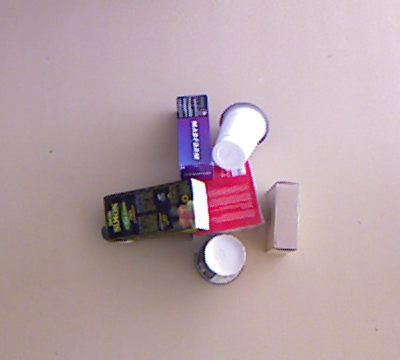
\includegraphics[width=\textwidth]{Img/ObjectSegmentation/seg1_rgb.png}
\end{subfigure}
\begin{subfigure}[t]{0.2\textwidth}
\centering

\includegraphics[width=\textwidth]{Img/ObjectSegmentation/seg1.png}
\end{subfigure}
\hspace{1.5cm}
\begin{subfigure}[t]{0.2\textwidth}
\centering
	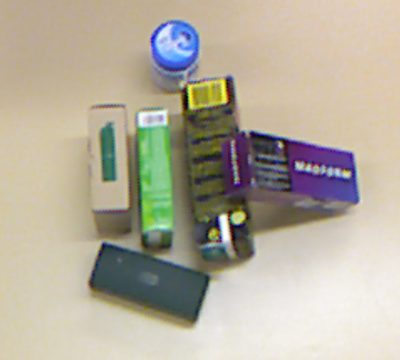
\includegraphics[width=\textwidth]{Img/ObjectSegmentation/seg3_rgb.png}
\end{subfigure}
\begin{subfigure}[t]{0.2\textwidth}
\centering
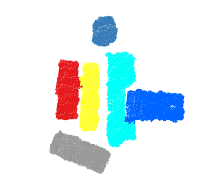
\includegraphics[width=\textwidth]{Img/ObjectSegmentation/seg3_original2.png}
\end{subfigure}
\caption{Example of segmentation results.}\label{fig:seg_results}
\end{figure}

Note that we set the algorithm in order to segment considering geometric properties, and not the color of the pixels. Considering the colors could lead to worst segmentation results for our case of studio since many objects have several colors.

\begin{wrapfigure}{r}{6.5cm}
\centering
\caption{Box with a green stripe.}\label{fig:seg_color}
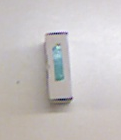
\includegraphics[width=3.5cm]{Img/ObjectSegmentation/color_seg_problem.png}
\end{wrapfigure}
A color based segmentation could segment a draw on an object, or a small part of the object, as a different object, but this, accordingly to the strategy we are going to use (see next sections), would lead to an unfeasible problem. 
For instance, in Figure \ref{fig:seg_color} is shown a box with a green stripe on its top surface, a segmentation algorithm based also on colors could lead to segment the green stripe as another object, and the result is that it is impossible to grasp the green stripe without collide with the box. This is the main reason the segmentation we used is based only on geometric features. 

\section{Background}
\label{sec:background_alg}
%\begin{itemize}
%\item collison detection
%\item pca
%\item table projection - convex hulls
%\item rotation matrices
%\end{itemize}

In this section some concepts, that will be used to execute the actions and to generate the states, are presented. 

\paragraph{Principal Direction}
The principal direction of an object is its principal axis which is defined as any of three mutually perpendicular axes about which the moment of inertia of a body is maximum. For instance, for a rectangular object its principal direction is the axis aligned with its longest dimension. 

To obtain the principal axis the principal component analysis (PCA) \citep{PCA} technique is used. This technique is a common statistical procedure that uses orthogonal transformation to convert a set of  observations of possibly correlated variables into a set of values of linearly uncorrelated variables, which are called principal components. The transformation is defined in a manner that the first component has the largest variance, the second has the second largest variance and so on. The principal components are orthogonal because they are the eigenvectors of the covariance matrix, which is symmetric. An example of the principal components for a 2D data set is depicted in Figure \ref{fig:pca1}\footnote{Image taken from \href{https://en.wikipedia.org/wiki/Principal_component_analysis}{https://en.wikipedia.org/wiki/Principal\_component\_analysis}}. The principal components are computed through the covariance matrix of the set of observation, and its eigenvectors $\bar{\lambda_v}$ represent the principal components while its eigenvalues $\lambda$ represent the variance of the data set along the principal component $\bar{\lambda_v}$. 

\begin{figure}[tb]
\centering
\begin{subfigure}[t]{0.45\textwidth}
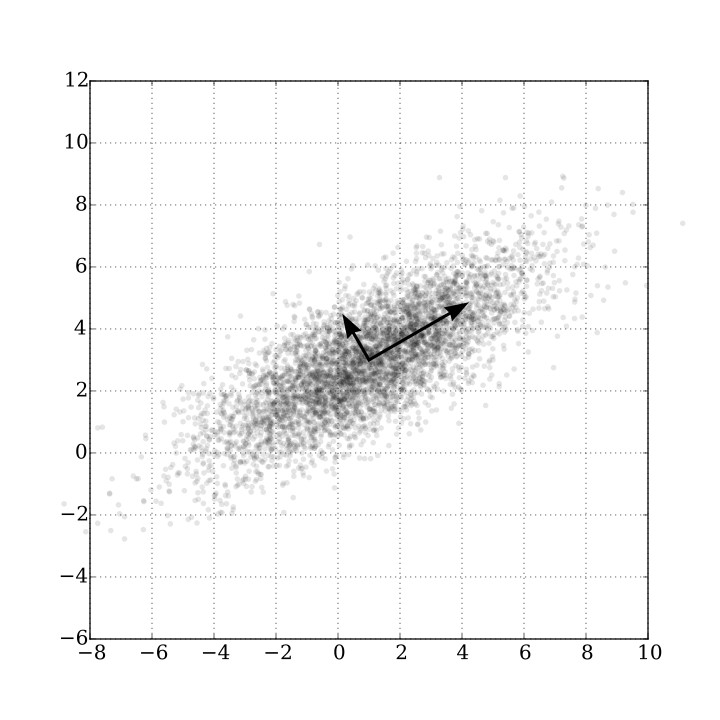
\includegraphics[width=\textwidth]{Img/pca/pca.png}
\caption{}\label{fig:pca1}
\end{subfigure}
\begin{subfigure}[t]{0.45\textwidth}
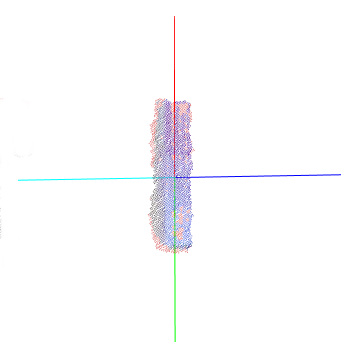
\includegraphics[width=\textwidth]{Img/pca/pca2.png}
\caption{}\label{fig:pca2}
\end{subfigure}
\caption{\textbf{Principal Components Analysis -} In Figure \ref{fig:pca1} PCA for a standard 2D set of observations. In Figure \ref{fig:pca2} results of the PCA for a rectangular segmented object. The \textcolor{green}{green}, \textcolor{red}{red} lines refers to different ways of the first principal direction, while \textcolor{blue}{blue} and \textcolor{cyan}{cyan} lines refers to different ways of the second principal direction. The third one is orthogonal to the first two principal directions.}
\end{figure}

A generic point cloud can be seen as a set of observations and the PCA can be directly applied to the object's point cloud to retrieve its principal components. In this works we refers to principal components as principal directions. In Figure \ref{fig:pca2} the first two principal directions of a generic object are illustrated. Note that for each principal direction we can actually obtain two directions (one per sense).

\paragraph{Projection onto a plane}
We will see later that the concept of the projections of a point into a plane will be useful. Considering a point $p=(x_p,y_p,z_p)$ and a plane $\mathcal{P}$ defined by the following equation
\begin{equation*}
a x + by + cz + d = 0
\end{equation*}
the projection $p_{\mathcal{P}}$ of point $p$ onto the plane $\mathcal{P}$ is given by the following set of operations:

\begin{enumerate}
\item Calculate the origin point $\mathcal{P}_O=(x_O,y_O,z_O)$ of the plane, which can be calculated by arbitrary $x_O$ and $y_O$ coordinates as
\[
z_O = \frac{-1}{c}(ax_O + by_O + d),
\]
then calculate the coordinates of $\mathcal{P}_O$ with respect the point $p$
\[
\mathcal{\prescript{p}{}P} = p - \mathcal{P}_O.
\]
\item Then calculate the projection of $\mathcal{\prescript{p}{}P}$ onto the plane normal $\bar{n}=(a,b,c)$
\[
\lambda_p = \bar{n} \cdot \mathcal{\prescript{p}{}P}. 
\]
%\item compute the coordinates of the projection onto the plane of point $p$ with respect to the point itself:
%\[
%p_P^p = 
%\]
\item Translate point $p$ by $\lambda_p$ along the normal of the plane $\bar{n}$
\[
p_P = p - \lambda_p \bar{n}. 
\]
The minus sign is due to the fact that the normal is pointing upwards.
\end{enumerate}

\paragraph{Rotation Matrices}
Rotation matrices express a rotation between two reference frames. Given two frames $\{A\}$ and $\{B\}$, and the rotation matrix $\prescript{A}{B}R$ that defines the rotation of $\{B\}$ relative to $\{A\}$ then a point $\prescript{A}{}P$ with respect frame $\{A\}$ is given by $\prescript{A}{}P=\prescript{A}{B}R\prescript{B}{}P$, where $\prescript{B}{}P$ is the same point relative to frame $\{B\}$. 

Having a frame $\{B\}$ defined by axis $\hat{\prescript{A}{}X_B},\hat{\prescript{A}{}Y_B}$ and $\hat{\prescript{A}{}Z_B}$, where $\hat{\prescript{A}{}Y_B}$ is the y axis of frame $\{B\}$ relative to frame $\{A\}$, the rotation matrix between $\{A\}$ and $\{B\}$ is defined as
\[
\prescript{A}{B}R = 
\begin{bmatrix}
\hat{\prescript{A}{}X_B} \\
\hat{\prescript{A}{}Y_B} \\
\hat{\prescript{A}{}Z_B} \\
\end{bmatrix}
\]
To transform any object, such as the gripper mesh model, to a pose defined by frame $\{B\}$ then the following homogeneous transform is applied:
\[
H = 
\begin{bmatrix}
\prescript{B}{A}R & \prescript{A}{}B_O \\
\bar{0} & 1
\end{bmatrix}
\]
where  $\prescript{B}{A}R={\prescript{A}{B}R}^{\top}$ and $\prescript{A}{}B_O$ is the origin of frame $\{B\}$ relative to $\{A\}$. In this way, having some axis that define our new reference frame, we can transform the gripper model in such a way its closing point is in the origin of the new frame and its orientation is aligned to the one of the new reference frame. 

\paragraph{Bounding Box}
A bounding box is the smallest cubic volume that completely contains an object\footnote{\href{https://en.wikipedia.org/wiki/Bounding_volume}{\url{https://en.wikipedia.org/wiki/Bounding\_volume}}}.
An axis-aligned bounding box (AABB) is a bounding box aligned with the axis of the coordinate system, while an oriented bounding box (OBB) is a bounding box oriented with the object. To compute the OBB the object is transformed from its frame to the world frame and the dimensions of the bounding box are obtained by computing the maximum and minimum coordinates of the transformed object. In this way it is possible to have an approximation of the length, width and height of an object.

\paragraph{Convex Hull}
A convex hull of a point cloud $P$ is the smallest 3D convex set that contains $P$. 
\begin{figure}[tb]
\centering
\begin{subfigure}[t]{0.3\textwidth}
\centering
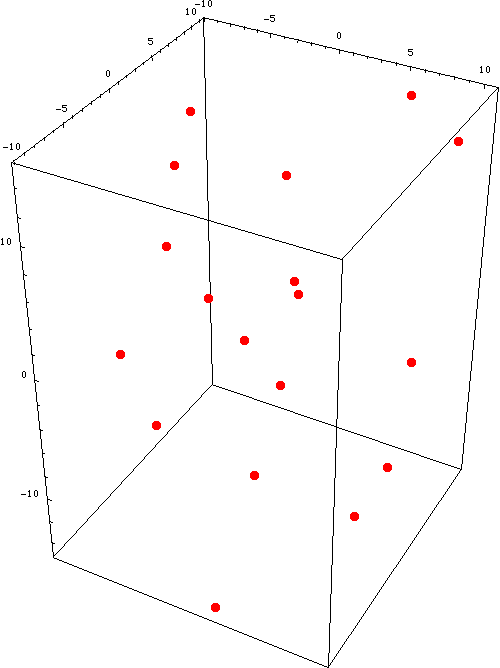
\includegraphics[height=4cm]{Img/convexhull/ch1.png}
\caption{Pointcloud}
\end{subfigure}
\begin{subfigure}[t]{0.3\textwidth}
\centering
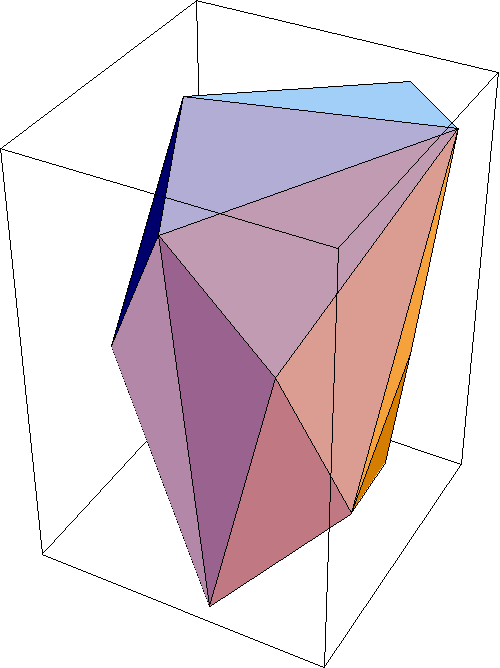
\includegraphics[height=4cm]{Img/convexhull/ch3.png}
\caption{Convex hull}
\end{subfigure}
\caption{Convex hull example}\label{fig:convexhull_example}
\end{figure}
In Figure \ref{fig:convexhull_example}\footnote{Images obtained from \href{http://xlr8r.info/mPower/gallery.html}{\url{http://xlr8r.info/mPower/gallery.html}}} an example of the convex hull for a point cloud is shown. The vertices are first detected and then connected among them by means of triangles. In this way a triangle mesh is associated to the convex hull. 

\paragraph{Collision Detection}
To understand if an object blocks a certain action, such as the pushing along a direction, we have to check if along the desired trajectory the pushed object will collide with the other ones. The collision detection is therefore a crucial step to generate the states. There exist different techniques to assert if two objects are colliding and all of them need a representation of the object, which could be a basic shape or a more complex as an octree. 

The mesh shape has been thought to use since it can be directly obtained from a convex hull. 

Given two objects A and B and their configurations $\bf{q_A}$ and $\bf{q_B}$, the collision test returns a boolean value about whether two objects collide or not \citep{pan2012fcl}. Two objects collide if
\[
A(\bf{q_A}) \cap B(\bf{q_B}) \neq 0
\]

The collision detection will be used to understand if in a given pose $\bf{q}$ the object $A$ would collide with the other objects in the scene.

In order to relax the collision detection majority of collision libraries, before to use complex algorithm to detect collision between two shapes, they first check if the bounding volumes (e.g. AABB) of the objects intersect, if they don't the objects surely don't collide. If their bounding volumes intersect the objects might collide.

\paragraph{Objects Modeling}
The Kinect can mainly see one face (usually the top) of the objects and therefore we cannot apply directly the convex hull algorithm to the detected surfaces. If we applied the convex hull on an object's observed surface, we would have likely the situation depicted in Figure \ref{fig:cv_top_collision}, in which the collision detections would not detect any collision when it should. This is because we are missing the surfaces that cannot be seen from the Kinect's point of view.

\begin{figure}[tb]
\centering
\begin{subfigure}[t]{0.3\textwidth}
\centering
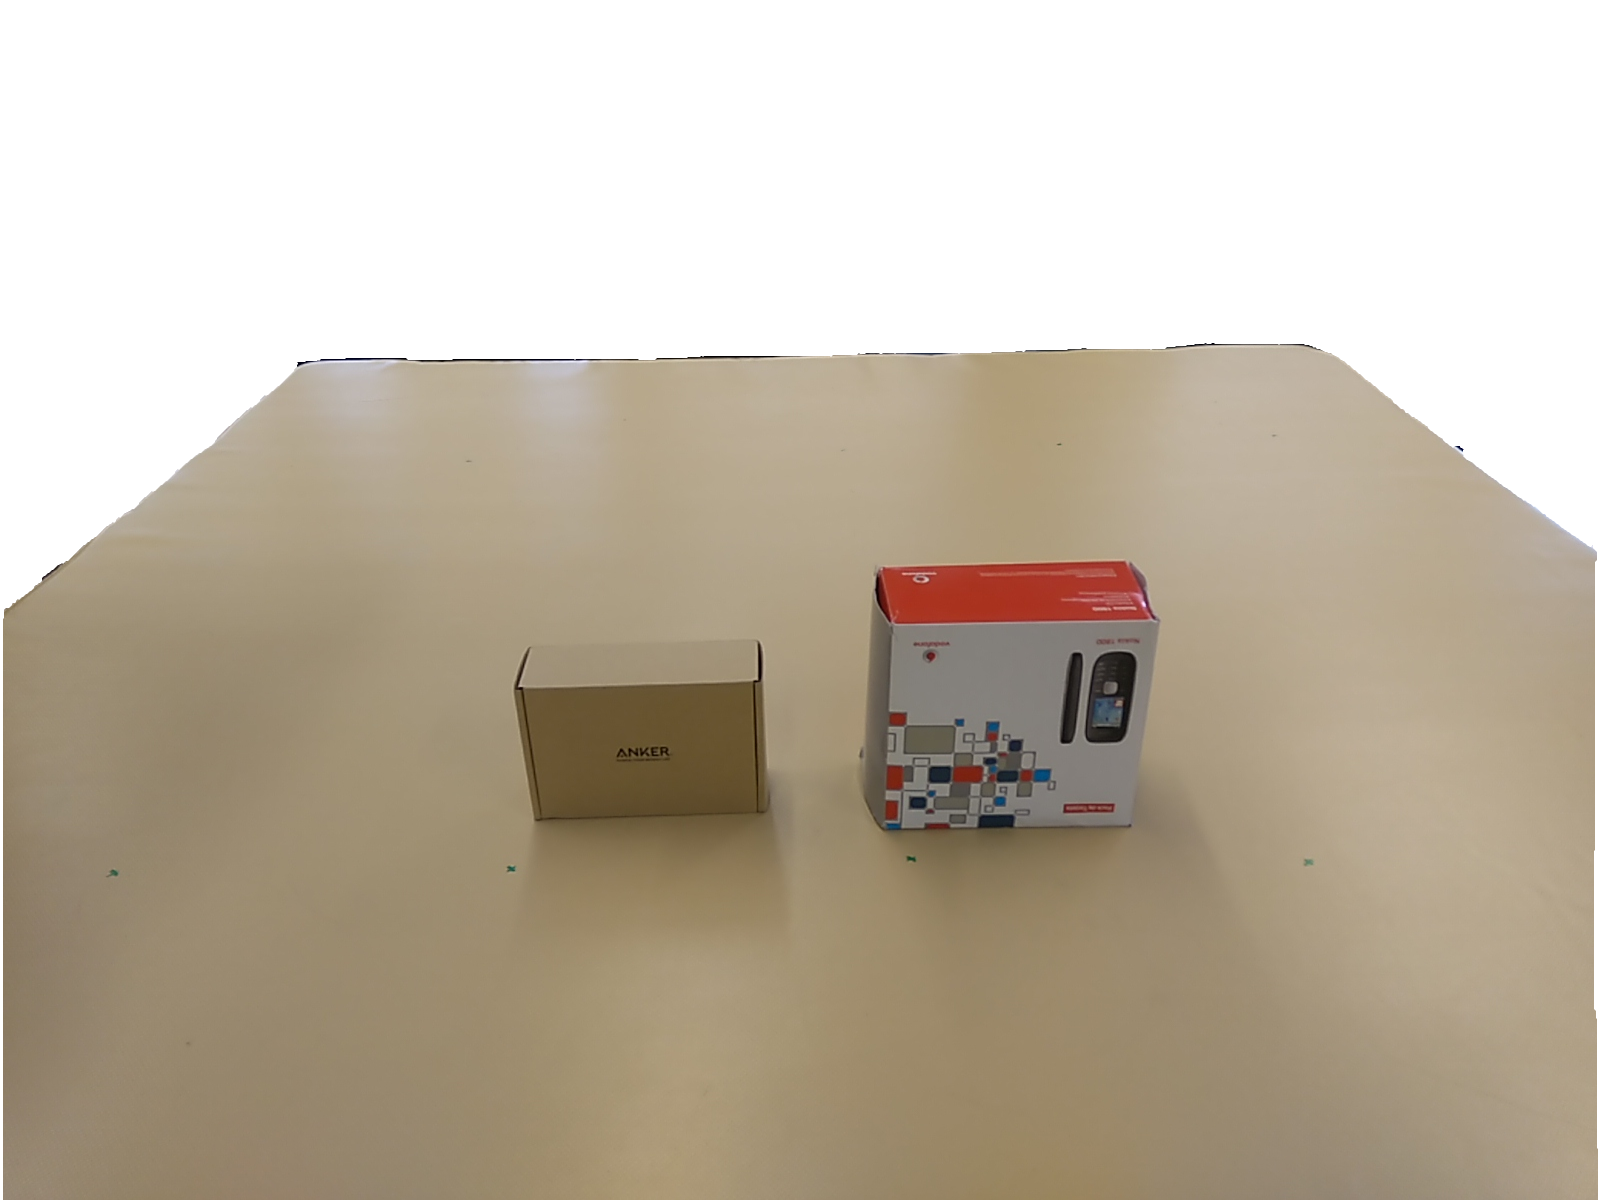
\includegraphics[width=0.9\textwidth]{Img/convexhull/example_only_top_surfaces.png}
\caption{}\label{fig:rgb_top_surfaces_example}
\end{subfigure}
\begin{subfigure}[t]{0.3\textwidth}
\centering
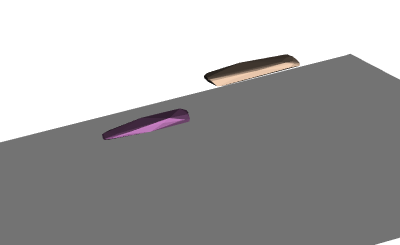
\includegraphics[width=0.9\textwidth]{Img/convexhull/cv_top2.png}
\caption{}\label{fig:cv_top}
\end{subfigure}
\begin{subfigure}[t]{0.3\textwidth}
\centering
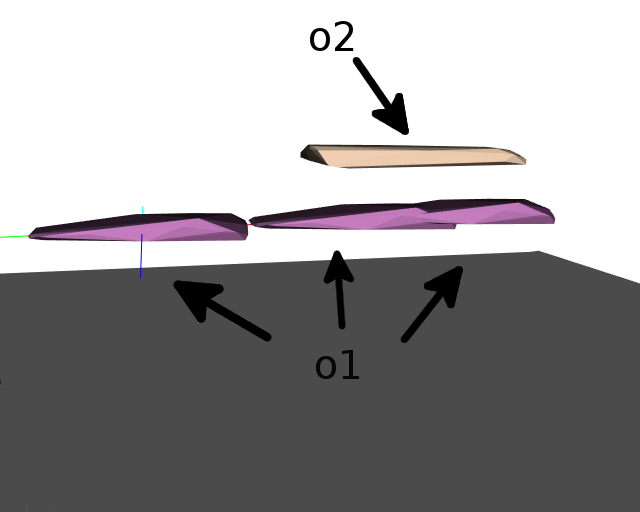
\includegraphics[width=0.9\textwidth]{Img/convexhull/cv_top_collision2.png}
\caption{}\label{fig:cv_top_collision}
\end{subfigure}
\caption{Convex hulls and collision detection using the segmented objects retrieved by the \ttt{LCCP} segmentation algorithm. The gray surface represents the plane's 2D convex hull. In Figure \ref{fig:cv_top} it is possible appreciating that we miss the information about the hidden part of the object. In Figure \ref{fig:cv_top_collision} a collision detection example is depicted. The convex hull of object \ttt{o1} is translated along a direction and no collision is detected  since the two convex hulls do not intersect.}
\end{figure}

From the Kinect's point cloud also the table plane is known, so the information we have are: the table plane model and the segmented objects (mainly the top surfaces).
If an human would be in the same pose of the Kinect, looking at the table, he would imagine that the objects are not floating surfaces, and he/she would deduce the objects shape from the shape of the top surface. The sides of the objects can be deduced by projecting the top surface's edges to the plane and then filling the missing object's sides with points. To do that we have to detect the top surface's edges. A easier method is directly projecting all the points of the surfaces onto the table plane and then apply the convex hull algorithm to the resulting point cloud given by the sum of the top surface and its projection. In this way the missing sides are indirectly retrieved by the convex hull. An example of this method is depicted in Figure \ref{fig:full_convexhull}.

\begin{figure}[tb]
\centering
\begin{subfigure}[t]{0.45\textwidth}
\centering
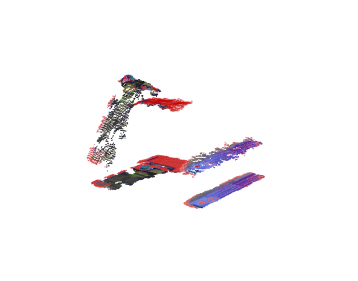
\includegraphics[width=0.9\textwidth]{Img/convexhull/projection.png}
\caption{Surfaces projection}\label{fig:projection}
\end{subfigure}
\begin{subfigure}[t]{0.45\textwidth}
\centering
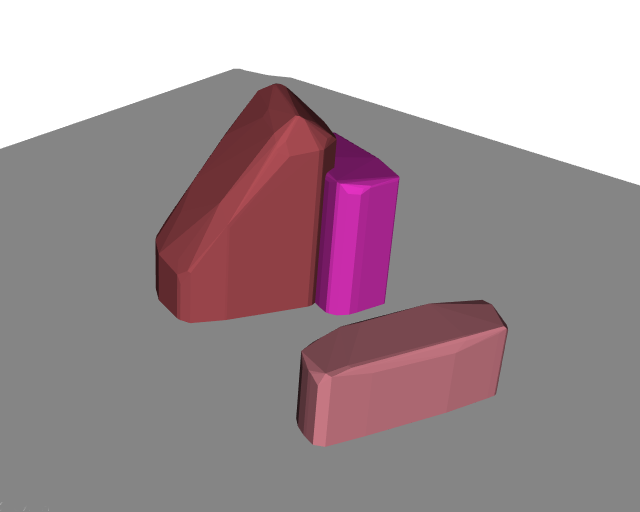
\includegraphics[width=0.9\textwidth]{Img/convexhull/full_convexhull2.png}
\caption{Resulting convex hull}\label{fig:full_convexhull_}
\end{subfigure}
\caption{Convex hull of the objects using their projections onto the table plane.}\label{fig:full_convexhull}
\end{figure}

%The PCL convex hull algorithm returns the convex hull as a triangular mesh, which can be used by the FCL for the collision detection. 

%The pose of the Kinect camera is above the table pointing forward it. In such a pose the Kinect is only able to see mainly the top side of the objects, and not their sides. 
%--- discussed the convex hull relating into to the neccesity for the collision detection.



\section{Action Execution}
Since the generation of the state depends on the way we decided to execute the actions, the way the actions are executed is discussed in this section.   

\subsection{Pushing}
\label{subsec:pushing}

Pushing is a difficult action to execute when the goal is to move one object along a path. The majority of pushing actions in object manipulation have the aim to interact with the objects in order to move them and validate the segmentation \citep{katz2014perceiving} \citep{katz2011interactive} \citep{Katz_2013_7407} , without taking care about the final position of the objects or about eventual collisions. Hermans er al. \citep{conf/iros/HermansRB12} presented a novel algorithm for object singulation through pushing actions, here the pushing actions have the aim to separate objects in cluttered scenes but they are not interested in singulate tidily the objects but just to find a feasible interaction to singulate them regardless possible collisions. 

%Grasping, although is a difficult task, has already an advanced state of the art regarding finding grasping pose also for complex objects. Somehow grasping is easier because it does not consider the whole object geometry but it is focused on looking for local futures that can be interesting for grasping the object (e.g. antipodal points). 

%When we push an object all the object's geometry has to be taken into account in order to find a suitable pushing direction. Moreover, humans push objects with a certain initial direction chosen accordingly the object geometry and then adapt the pushing direction accordingly to the error with respect the desired one. This would imply the implementation of a controller which is out the scope of this thesis. 

Inspired by this consideration, we decided to consider its first two principal directions as possible directions to push an object. In particular, there are two senses for each direction, so in total we have 4 possible pushing directions per object, as depicted in Figure \ref{fig:directions}.

\begin{figure}
\centering
\begin{subfigure}[t]{6cm}
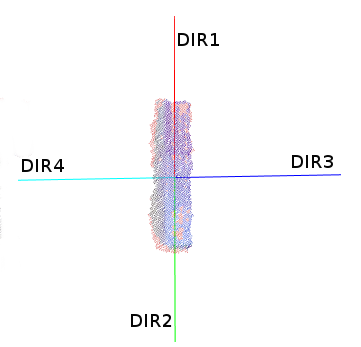
\includegraphics[width=5.5cm]{Img/pushing/directions.png}
\caption{Pushing directions computed using the segmented surface seen by the Kinect.}\label{fig:directions1}
\end{subfigure}
\quad
\begin{subfigure}[t]{6cm}
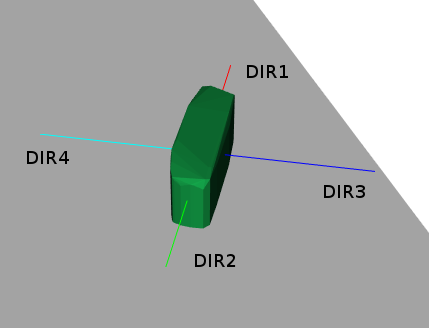
\includegraphics[width=5.5cm]{Img/pushing/directions2.png}
\caption{Pushing directions associated to the object's convex hull.}
\label{fig:directions2}
\end{subfigure}
\caption{Example of pushing directions.}\label{fig:directions}
\end{figure}


Another things to take into account is that the principal directions are not always parallel to the table plane. An object which stands on top of a table will be obviously pushed along a direction parallel to the table. For this aim the first two principal directions are projected on to the table plane. So the pushing directions considered are not the principal directions but their projections. 

%Another thing to take into account is that the principal directions are not always parallel to the table plane. An object which stands on top of a table will be obviously pushed along a direction parallel to the table. As previously described in Section \ref{sec:background_alg} a point can be projected on to the table plane, but a point and a vector (the principal directions are vectors) have the same representation, and therefore we can apply exactly the same equations to obtain the projections of the principal components onto the table plane. So the pushing directions considered are not the principal directions but their projections. 

Next, the pose of the gripper is computed accordingly to its shape, to the shape of the objects and the pushing direction.

%Next, having some pushing directions along with the robot will push the object, the pose for the the gripper to push that object has to be decided. The pose has been chosen accordingly to the shape of the gripper.\DMcomment{Rewrite this paragraph}

In Figure \ref{fig:gripper_side}
%is possible observing the profile of the gripper mounted to the base of the gripper, highlighted by the blue color. Such base has a circular shape and the gripper's deep is less then the one of the base. It is undesirable pushing an object with a circular, or spherical, shape for the end effector because there is more uncertainty on the resulting path of the manipulated object. The gripper has no a circular shape and it is symmetric, this make it suitable to push an object with a certain stability (i.e. make the object follow the desired path) during the action. 
is possible observing the profile of the gripper mounted to the base of the gripper, highlighted by the blue color. Such base has a circular shape and the gripper's depth is less than the one of the base. It is undesirable pushing an object with a circular, or spherical, shape for the end effector because there is more uncertainty on the resulting path of the manipulated object. The gripper has no a circular shape and it is all symmetric, this make it suitable to push an object with a certain stability (i.e. make the object follow the desired path) during the action. Since we want a pushing action as accurate as possible, we don't want that the gripper's base touches the manipulated object. 

\begin{figure}[tb]
\begin{subfigure}[t]{0.25\textwidth}
\centering
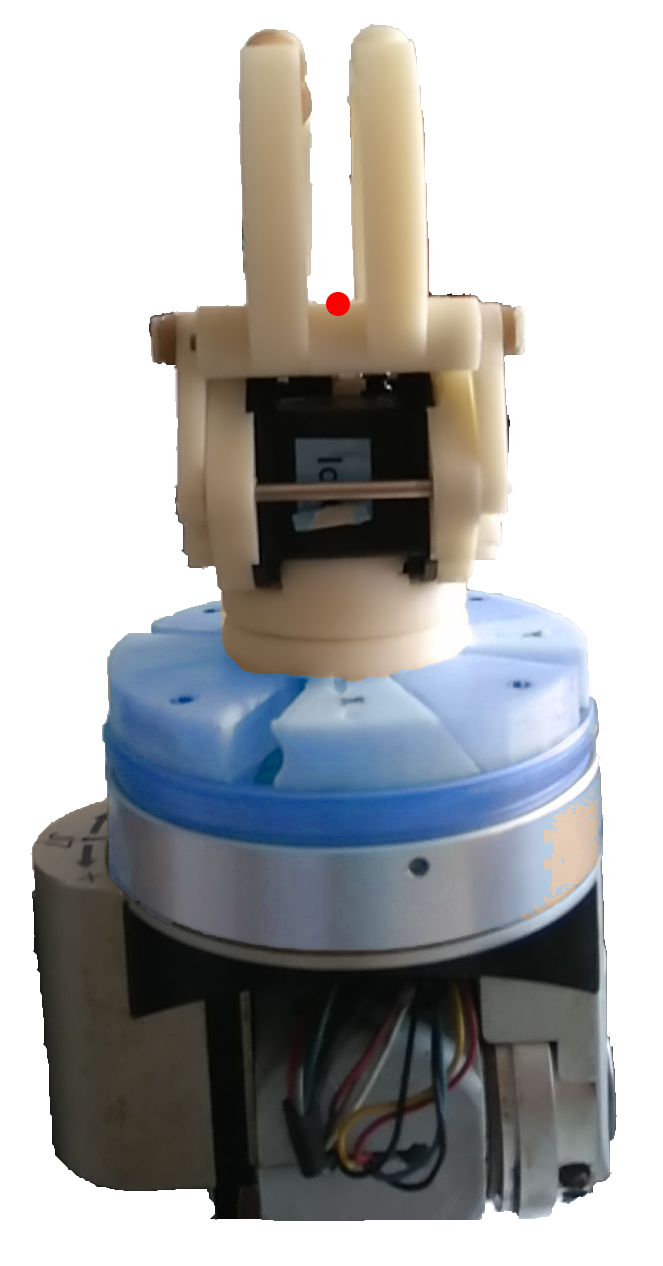
\includegraphics[width=2.5cm]{Img/set_up/gripper_side2.png}
\caption{The gripper and its base.}\label{fig:gripper_side}
\end{subfigure}
\begin{subfigure}[t]{0.7\textwidth}
\centering
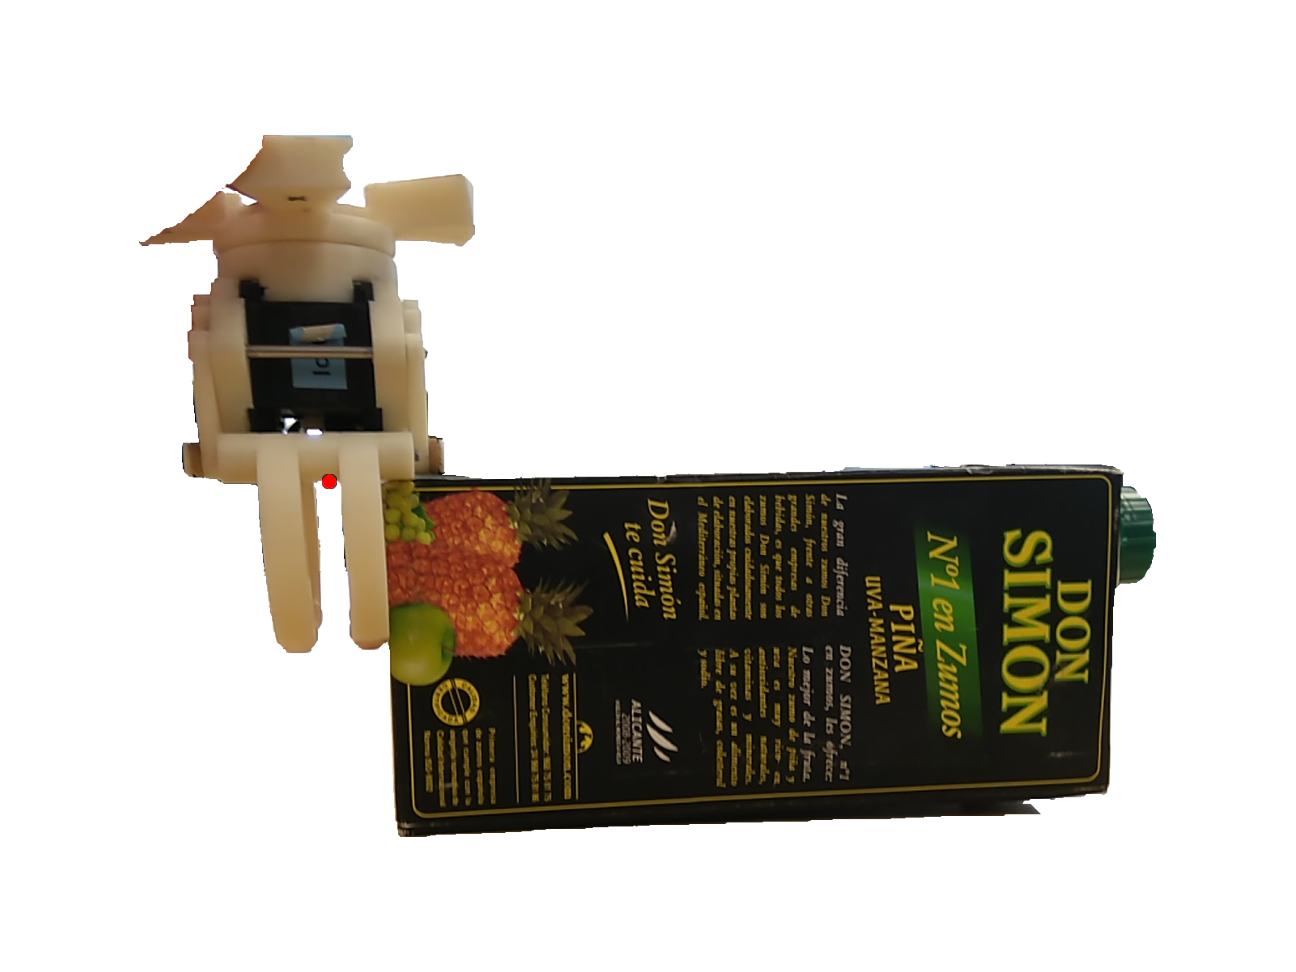
\includegraphics[width=7cm]{Img/pushing/pushing1.png}
\caption{Profile view of a desired pose for pushing an object.}\label{fig:pushing_pose}
\end{subfigure}
\caption{}
\end{figure}


%Due to the limited opening width of the gripper (7 centimetres) the object the robot is going to manipulate have small width. This means that when pushing along the principal axis, the object's width is likely small. Such a situation is depicted in Figure \ref{fig:pushing_way1}. Pushing in such a way the gripper will likely push also the black juice box. Therefore when pushing along the principal axis the pose is chosen to be the one in Figure \ref{fig:pushing_way2}. Of course is more stable a pushing pose like the one in Figure \ref{fig:pushing_way1}, since the contacts point (the fingers) are more distant. For this reason that pose is used only when pushing the objects along a direction 3 and 4.

Knowing also the height of the objects retrieved by its OBB, it is possible having a pose for the gripper is such a way that the gripper's base does not touch the object. The gripper's pose, relative to the object, is computed in manner to locate the red point of Figure \ref{fig:gripper_side} to be at the same height of the object. In this way the fingers will fully touch the object during the pushing action. Moreover, to make easy for the robot reaching the pushing pose, it was defined to be a certain distance from the object (in our experiment it was set to 5cm). It would be difficult to reach a pose of Figure \ref{fig:pushing_pose} without colliding with the object.  

Due to the limited opening width of the gripper (7 centimetres) the objects the robot can manipulate are thin. This means that when pushing along the principal axis, the object's width is likely small(Figure \ref{fig:pushing_way1}). Pushing in such a way the gripper will likely push also the black juice box. Therefore when pushing along the principal axis, the pose used is the one in Figure \ref{fig:pushing_way2}. The pose of Figure \ref{fig:pushing_way1} is more stable since the contacts point (the fingers) are more distant between themselves. For this reason this pose is used only when pushing the objects along a direction 3 and 4.


\begin{figure}[tb]
\centering
\begin{subfigure}[t]{0.45\textwidth}
\centering
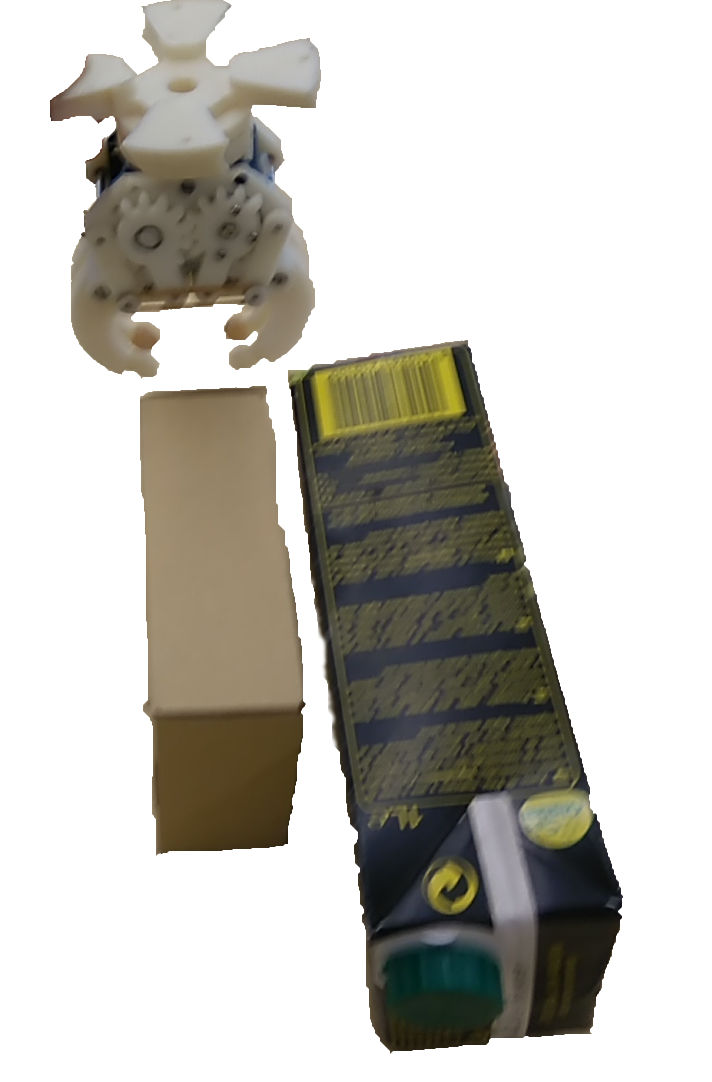
\includegraphics[width=3cm]{Img/pushing/pushing333.png}
\caption{}\label{fig:pushing_way1}
\end{subfigure}
\begin{subfigure}[t]{0.45\textwidth}
\centering
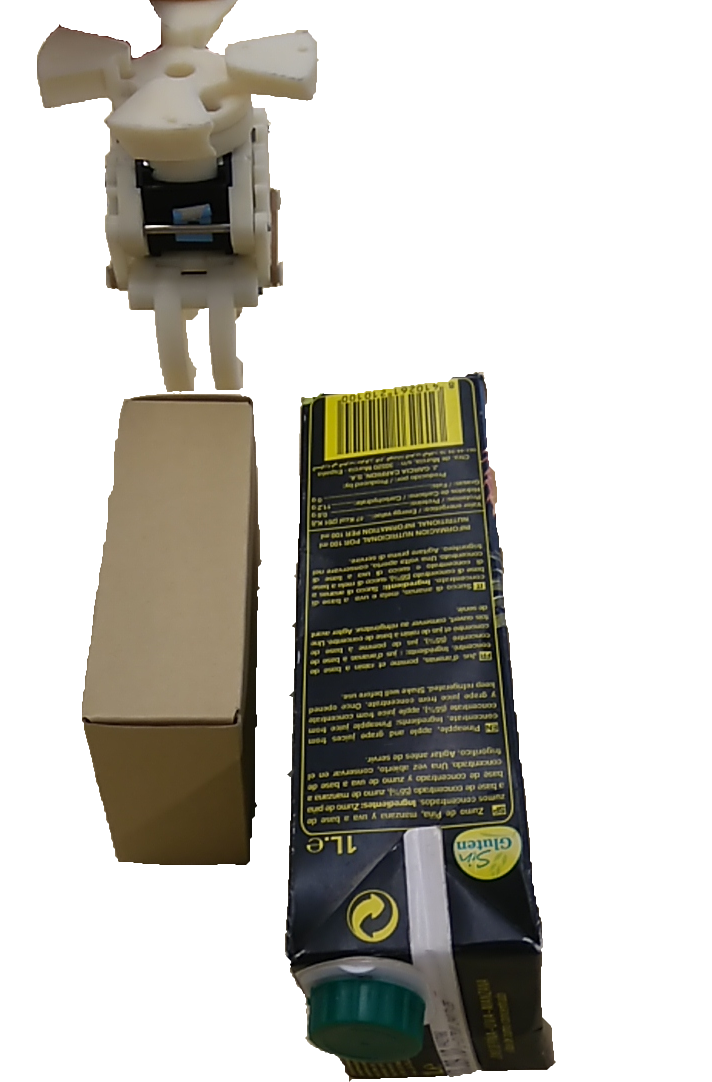
\includegraphics[width=3cm]{Img/pushing/pushing222.png}
\caption{}\label{fig:pushing_way2}
\end{subfigure}
\caption{\textbf{Possible pushing poses for push an object along its principal axis} - In Figure \ref{fig:pushing_way1} the closing direction of the gripper is orthogonal to the pushing direction, and for the case depicted in the figure the gripper will likely push also the black juice box. In Figure \ref{fig:pushing_way2} the closing direction of the gripper is parallel to the pushing direction.}\label{fig:pushing_way}
\end{figure}

Having the projections of the principal components, the table normal and the desired coordinates for the gripper's closing point it is possible defining a rotation and translation matrices. To push along direction 1 those matrices are:

\begin{equation}
R_{dir1} =
\begin{bmatrix}
dir2_X & dir2_Y & dir2_Z \\
dir4_X & dir4_Y & dir4_Z \\
n_x & n_y & n_z \\
\end{bmatrix}^{\top}
\qquad \qquad
T=
\begin{bmatrix}
c_x \\ c_y \\ c_z
\end{bmatrix}
\label{eq:transform}
\end{equation}
where $dir1_X$ refers to the x coordinate of the vector that defines the direction 1, $n$ is the table normal and $c$ is the desired tool closing point\footnote{The gripper's closing point is finger's contact point. (Although in this case the fingers do not touch themselves)}. 
% The rotation matrix $R_{dir3}$ for pushing along direction 3 would be the same of $R_{dir1}$. 


%As previously said, the planner considers to push the objects at infinity, in the reality the robot has to push the objects for a finite length. Since the planner has no geometric information, the pushing length is chosen accordingly the dimension of the AABB relative to the pushing direction. For instance, if the robot is going to push the object \ttt{o1} along direction 1 the length $l$ of the pushing action is $l=k \cdot AABB_{\mathtt{o1}}(length)$, where $k$ is a gain factor (1 in our experiments) called \textit{pushing step}. This is a limitation since the robot will push an object for a length which is function of the manipulated object and not to surrounding ones. 

As previously said, the planner considers to push the objects at infinity, but in reality the robot has to push the objects for a finite length. Since the planner has no geometric information, it does not know how much it has to push in order to singulate the object, or to make it graspable. For this reason the pushing length is chosen accordingly the dimension of the OBB relative to the pushing direction. For instance, if the robot is going to push the object \ttt{o1} along direction 1} the length $l$ of the pushing action is $l=k \cdot OBB_{\mathtt{o1}}(length\_object)$, where $k$ is a gain factor (1 in our experiments) called \textit{pushing step}. This is a big limitation since the robot will push an object for a length which is function of the manipulated object and not of the surrounding ones. The improvement of this limitation will be one of the topics for future works.


To retrieve the path we consider the total length $l$ and we discretize it by $n$ points having in this way $n+2$ poses ($+2$ because of the pushing pose and the final pose). For each pose the inverse kinematic is calculated. In this way we obtain a discrete path. 

When the robot approaches the pushing pose it could be that it collides with other objects. It would be suitable to use \textit{MoveIt!}\footnote{Ioan A. Sucan and Sachin Chitta, “MoveIt!”, [Online] Available:\href{http://moveit.ros.org} {\url{http://moveit.ros.org}}} which can build an octomap representation of the scene and find a path avoiding collisions with the scene. The integration of \textit{MoveIt!} will be a future work. To avoid the collisions we considered a pre-pushing pose which has the same pose of the pushing pose but translated, accordingly to the table's normal, $20$ centimetres from the pushing pose. This pre-pushing pose is easier to reach without collisions. 
After the execution of the pushing action the robot goes to its \textit{home} pose (depicted in Figure \ref{fig:setup_}) in order not to stay inside the Kinect's view. When it goes to home it might happen that it collides with some objects, so also for the final pose we considered another one translated, accordingly the table normal, $20$ centimetres from the last pose. 
In this way the pushing trajectory is defined by a total of $n+4$ poses. 


%Note that we can obtain with this method is:
%\begin{itemize}
%\item pushing direction for simple objects: we can push the rectangular object of Figure \ref{fig:pca2} along one of the ways of the first two principal directions, 
%\item assign a reference frame to the object: by using the three principal components we can obtain a new reference frame $F_{o_i}$ for each object.
%\end{itemize}

%The computed principal components are orthogonal between themselves but the way of eigenvector $\bar{\lambda}$ is chosen by the PCA algorithm. In our case we are interested having a coherent description of the pushing directions as indicated in Figure \ref{fig:pca2}, and for that aim $\bar{\lambda_2}$ has to be always the same way with respect to the first principal component $\bar{\lambda_1}$. 

\subsection{Grasping}
\label{sec:grasping}
%\todo[inline]{Review of grasping techniques}
%\textbf{ROS object\_manipulator}\\

There exist an advanced state of the art regarding grasping. Despite this, all the techniques of grasping are usually computationally expensive. Many of them rely on the identification of the shape of the objects and then a set of pre-built grasping poses is returned\citep{brook2011collaborative}. Other techniques rely on the identification of local features which can state if a grasping pose is feasible or not. Two goods grasping planning algorithms of this kind, which deal with novel objects, are AGILE \citep{AGILE} and HAF \citep{haf}, despite this, they are not so robust and they are computationally expensive and not suitable for this thesis \citep{covallero}. In order to have a fast planning algorithm we considered a very simple approach to grasp the objects, which is suitable only with the kind of objects we are going to interact with. Despite this, the planner presented by this thesis can be directly integrated with several grasping algorithms. 

The idea is to grasp the object in manner that the gripper's closing direction\footnote{The gripper's closing direction is the direction along with the fingers move when grasping.} is orthogonal the principal axis of the object. The approaching direction\footnote{The gripper's approaching direction is the direction along with the gripper approaches the grasping pose.} of the gripper is given by the third principal component of the object. Then the gripper's closing point coordinates are given by the centroid, of the object's top surface, translated along the approaching direction by the half of the gripper's fingers height.
In this manner a single grasping pose is obtained for each object. 

To grasp the object also the robot needs a pre grasping pose, if not the gripper would collide with object attempting to reach the grasping pose, moving it away, and the grasp would fail. The pre grasping pose is simply defined by the grasping pose translated along its approaching direction by $10$ centimetres.
Once the object has been grasped it is easy that it collides with other ones, therefore a post grasping pone is defined by translating the grasping pose for $20$ centimetres along the table's normal.

On the whole the grasping action is composed of the following set of actions: 
\begin{enumerate}
\item Reaching the pre grasping pose.
\item Opening gripper.
\item Reaching grasping pose.
\item Closing gripper.
\item Reaching the post grasping pose again.
\item Going to the dropping pose: the object will be dropped into a bin.
\end{enumerate}


\section{States generation}
In Chapter \ref{ch:planning_system}  the predicates used were described, in this section their computation is presented in detail. 

\subsection{Predicate: \texttt{block\_grasp}}
The \ttt{(block\_grasp o1 o0)} predicate refers to the fact that object \ttt{o1} blocks \ttt{o0} to be grasped. The computation is this predicate is straightforward: the mesh model of the opened gripper is transformed to the grasping pose of object \ttt{o0}, and checked if it collides with the other objects. In figure \ref{fig:block_grasp} such procedure is shown and in Algorithm \ref{alg:block_grasp} the pseudo algorithm is described in detail. 

\begin{figure}[tb]
\centering
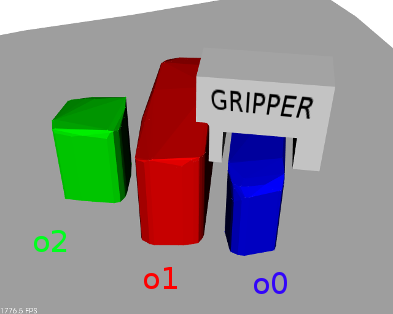
\includegraphics[width=6.5cm]{Img/grasping/block_grasp.png}
\caption{Visualization of the computation of \texttt{block\_grasp} predicate for object \ttt{o0}. The opened gripped model is transformed to the grasping pose for object \ttt{o0} and it is tested if the gripper mesh model collides with the other objects, in this case it collides with \ttt{o1}. }\label{fig:block_grasp}
\end{figure}

\begin{algorithm}
\caption{Computation of \texttt{block\_grasp} predicates. \\
\textbf{Inputs:} Set of objects $O$ (convex hull retrieved with the projection onto the table plane) and  the set of grasping poses $G_{poses}$.\\
\textbf{Outputs:} The \ttt{block\_grasp} predicates.
}\label{alg:block_grasp}
\begin{algorithmic}
\Function{ComputeBlockGraspPredicates}{$O$,$G_{poses}$}\\
  \texttt{block\_grasp\_predicates} $\gets$ \textsc{NULL}
\ForAll{$A \in O$}
  \State $gripperMeshTransformed \gets$ \textsc{trasnformGripperModel}($G_{poses}(A)$)
\ForAll{$B \in O$}
  \If{$A \neq B$} 
	\State $collision \gets$ \textsc{isThereCollision($gripperMeshTransformed$,$B$)}
	\If{$collision$}
		\State \texttt{block\_grasp\_predicates} $\gets$ \textsc{AddPredicate}(\texttt{(block\_grasp B A)})
	\EndIf
  \EndIf
\EndFor
\EndFor \\
\Return  \texttt{block\_grasp\_predicates}
\EndFunction
\end{algorithmic}
\end{algorithm}   
 
%Notice that this method implies to check for collision between the gripper and objects that might be very far from the interested object, i.e. there is no need to compute the collision detection.  Despite this, as explained in Section \ref{sec:background_alg}, the majority of collision detection algorithms first check if the bounding boxes of the objects intersect. This is a computationally cheap operation, and only if they intersect the computationally expensive algorithm are used to check for collision. This makes the Algorithm \ref{alg:block_grasp} efficient and computationally not expensive. It has been observed that, in average, to compute this predicate the time is about $10$ milliseconds per object and the complexity to compute this state is $\mathcal{O}(n^2)$, where $n$ is the number of objects.

Notice that this method requires to check for collision between the gripper and objects that might be very far from the interested object, i.e. there is no need to compute the collision detection.  Despite this, as explained in Section \ref{sec:background_alg}, the majority of collision detection algorithms first check if the bounding boxes of the objects intersect. This is a computationally cheap operation, and only if they intersect the computationally expensive algorithm are used to check for collision. This makes the Algorithm \ref{alg:block_grasp} efficient and computationally not expensive. It has been observed that, in average, to compute this predicate the time is about $10$ milliseconds per object. 
 
\subsection{Predicate: \texttt{on}}
The \ttt{(on o0 o1)} predicate means that object \ttt{o0} is on top of object \ttt{o1}. With the convex hull of the objects is easy to understand if two objects are one on top of the other one by checking for collision, but in this way we do not know who is above and who is below. To do this their surface projections onto the table plane are used. 
The research group of Artificial Intelligence and Robotics Laboratory of
Istanbul Technical University, published some interesting researches suitable to the aim of this thesis. In \citep{ersen2014scene} \citep{SSS147762} \citep{ersen2013extracting} the authors proposed some approaches to enhance
 3D recognition and segmentation results to create and maintain a consistent world model involving attributes of the objects and spatial relations among them. Their researched focused on modelling the world for manipulation planning tasks. They do not consider scene like the one of this thesis but simpler ones such as  a pile of cubes above each other. What can be directly used from their work is the computation of the \ttt{on} predicate. The \textit{on} relation for a pair of objects is determined by checking whether their projections onto the table plane overlap. This predicate was not a relevant part of their work and they did not provide too much information about its computation. Therefore our implementation for the \ttt{on} predicate is based on their idea with some modifications. 
 
Our idea is based on the fact that an object which stands on top of another one occludes some parts of the object below. In the other side, the one below does no occlude any part of the top object. 
Let's consider the scene in Figure \ref{fig:on_predicate_original}, the object \ttt{o0} occludes a portion of object \ttt{o1}. The projections ${\sc P_{0}}$ and ${\sc P_{1}}$ onto the table plane of \ttt{o0} and \ttt{o1} are respectively the red and green ones in Figure \ref{fig:on_1}. The convex hull ${\sc C_{P_{1}}}$ of the projection $P_{1}$ of \ttt{o1} intersects with the projection ${\sc P_{0}}$ of \ttt{o0}, while the projection ${\sc P_{1}}$ of \ttt{o1} does not interesct with the convex hull ${\sc C_{P_{0}}}$ of the projection of \ttt{o0} (Figures \ref{fig:on_2} and \ref{fig:on_3}). 


\begin{figure}[tb]
\centering
\begin{subfigure}[t]{0.45\textwidth}
\centering
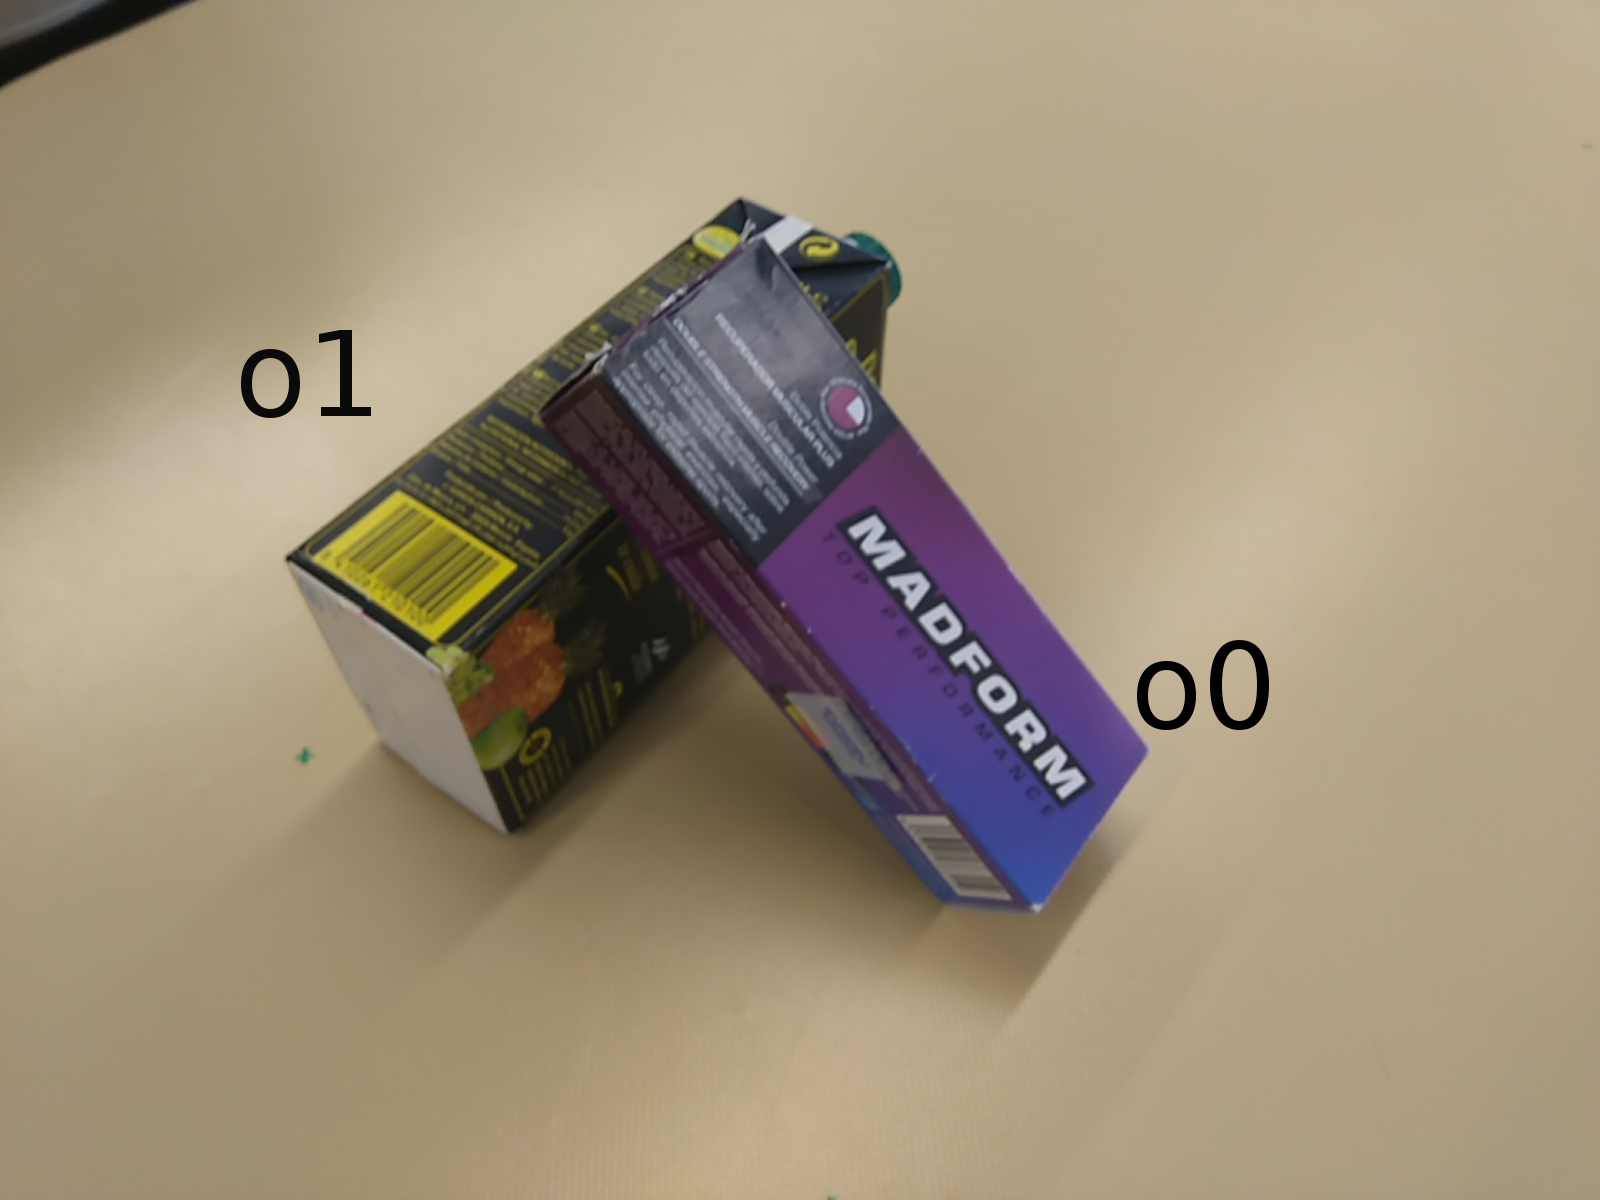
\includegraphics[width=5cm]{Img/on/on1.jpg}
\caption{Scene}\label{fig:on_predicate_original}
\end{subfigure}
\begin{subfigure}[t]{0.45\textwidth}
\centering
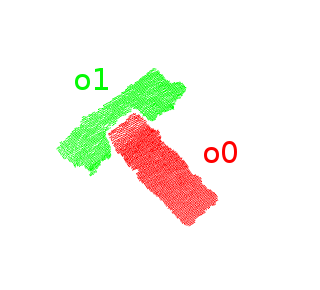
\includegraphics[width=5cm]{Img/on/on2.png}
\caption{$P_0 \quad \& \quad P_1$}\label{fig:on_1}
\end{subfigure}
\begin{subfigure}[t]{0.45\textwidth}
\centering
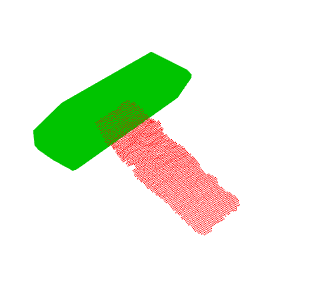
\includegraphics[width=5cm]{Img/on/on4.png}
\caption{${\sc C_{P_{1}}} \quad \& \quad {\sc P_{0}}$}\label{fig:on_2}
\end{subfigure}
\begin{subfigure}[t]{0.45\textwidth}
\centering
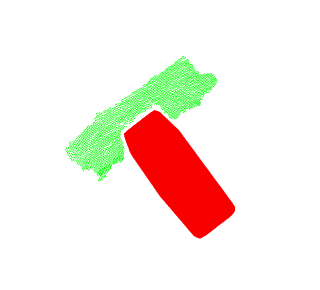
\includegraphics[width=5cm]{Img/on/on3.png}
\caption{${\sc C_{P_{0}}} \quad \& \quad {\sc P_{1}}$}\label{fig:on_3}
\end{subfigure}
\caption{Visualization of the computation of the \ttt{on} predicate. Figure \ref{fig:on_1} shows the real image, Figure \ref{fig:on_1} shows the projections of the objects onto the table plan while Figures \ref{fig:on_2} and \ref{fig:on_3} represent the two steps strategy to compute the \ttt{on} predicate.}\label{fig:on_predicate}
\end{figure}

Although this method works fine to compute the \ttt{on} predicate it has the limitation that its scope is only for objects for a rectangular shape, or similar shapes.

It is important to take into account also that actually the edges of the occluded parts of the below object, once projected, could be at the same position, of some projected edges of the top object. This could be dangerous for the computation of this predicate. Therefore a threshold is added. Focusing the attention on Figure \ref{fig:on_2} it can be appreciated that the intersection ${\sc C_{P_{1}}} \cap {\sc P_{0}}$ includes several points, while, in case the edges projections relative to the occluded and occluding part have similar coordinates, the intersection ${\sc C_{P_{0}}} \cap {\sc P_{1}}$ would include just few points. Therefore the \ttt{(on o0 o1)} predicate is update accordingly to the following formula:
\begin{equation}
\ttt{(on o0 o1)} =
\begin{cases}
{\sc True}, \qquad length({\sc C_{P_{0}}} \cap {\sc P_{1}}) < th_0 \;\; \wedge \;\; length({\sc C_{P_{1}}} \cap {\sc P_{0}}) > th_1 \\
{\sc False}, \qquad otherwise
\end{cases}
\label{eq:on}
\end{equation}
where $length(A)$ means the number of elements in the set $A$.
The values of the thresholds $th_0$ and $th_1$ are determined empirically and they are $th_0=th_1=100$.

The formula \ref{eq:on} is then evaluated for every possible combinations of objects, therefore the complexity to generate this state is $\mathcal{O}(n^2)$, where $n$ is the number of objects. Despite this, its computation is very fast. The example in Figure \ref{fig:on_predicate} was evaluated just 2 times since there are only 2 objects and it took $3$ milliseconds, that is $\approx 1.5 \frac{ms}{pair \; of \; object}$. For instance, for a complex scene with 10 objects the total time devoted to compute this predicate would be approximatively $10 \cdot 9 \cdot 1.5 \approx 135 ms$.



\subsection{Predicate: \texttt{block\_dir$_i$}}
The \ttt{(block\_dir$_i$ o1 o0)} predicate, if true, means that object \ttt{o1} blocks object \ttt{o0} when moved along its $i$-th direction. 

Object \ttt{o1} can blocks object \ttt{o0} to be moved along a certain direction if a collision will appear between the two objects. In order to do that, having a certain pushing length $l_i$ for the $i$-th direction of object \ttt{o0}, its convex hull $C_{\mathtt{o0}}$ is translated along the considered direction until reaching its final position which is $p_f=p_i + l \cdot dir_i$, where $p_f$ and $p_i$ are respectively the centroid at the final and initial pose. Object \ttt{o0} is going to do a path from its initial and final pose so the collision should be checked along its path. 
%To do that we could use a continuous collision detection algorithm or a discrete one. The continuous method suppose that given an object, its initial, its final pose and the other objects in the environment it will detect a collision if a collision occurs from the initial to the final pose. This algorithm has the advantage to be accurate but we should repeat it separately for each object since we are not interested to see if there is a collision, but we are interested in knowing what is the object it is going to collide with. 
We decided to use a discrete strategy, that is we consider several poses between the initial one and the final one, including the final one, and for each one we check if the transformed object collides with the other objects. 



\begin{figure}[tb]
\centering
\begin{subfigure}[t]{5cm}
\centering
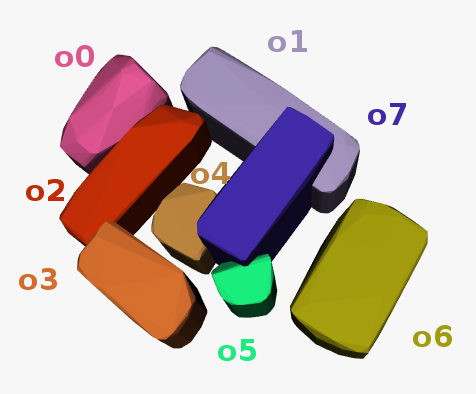
\includegraphics[width=5cm]{Img/block_dir/original_labels2.png}
\caption{Top view of the convex hull of the segmented objects.}\label{fig:block_dir_original}
\end{subfigure}
\begin{subfigure}[t]{5cm}
\centering
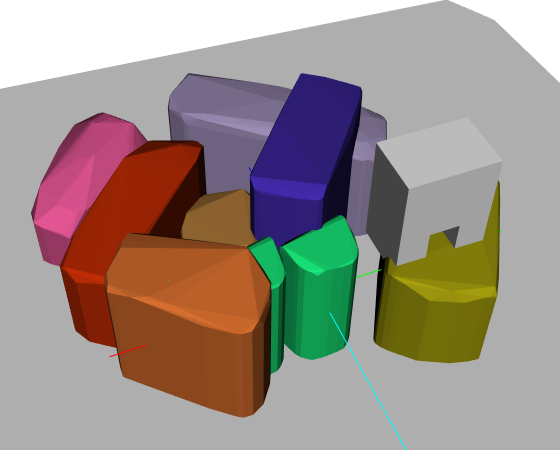
\includegraphics[width=5cm]{Img/block_dir/pushing11.png}
\caption{Evaluating the \ttt{(block\_dir1 * o5)} predicate}\label{fig:block_dir_push1}
\end{subfigure}
\begin{subfigure}[t]{5cm}
\centering
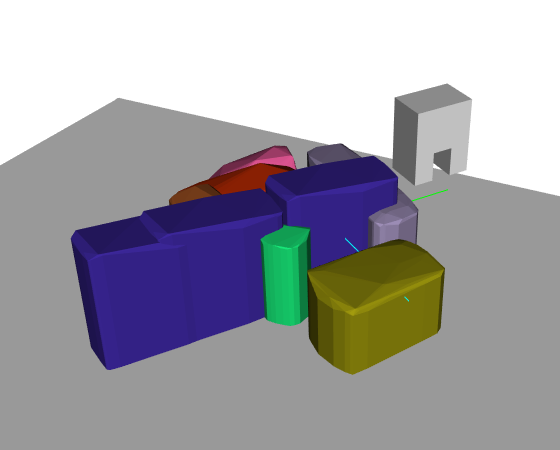
\includegraphics[width=5cm]{Img/block_dir/pushing22.png}
\caption{Evaluating the \ttt{(block\_dir1 * o7)} predicate}\label{fig:block_dir_original}
\end{subfigure}
\begin{subfigure}[t]{5cm}
\centering
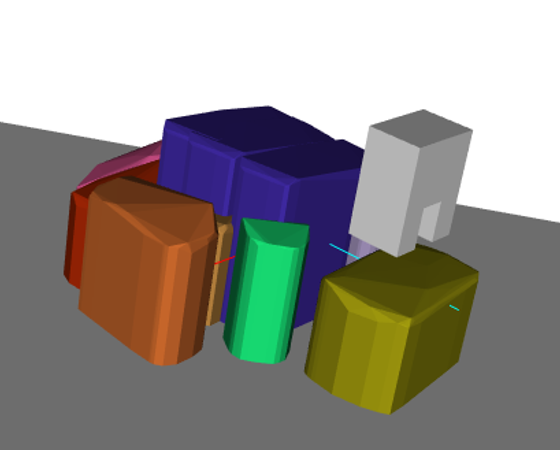
\includegraphics[width=5cm]{Img/block_dir/pushing33.png}
\caption{Evaluating the \ttt{(block\_dir3 * o7)} predicate}\label{fig:block_dir_original}
\end{subfigure}
\begin{subfigure}[t]{5cm}
\centering
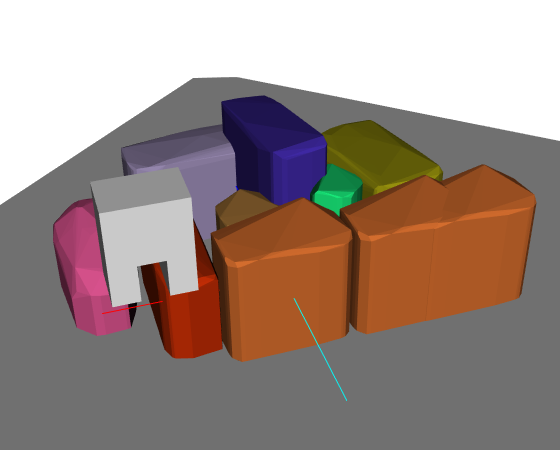
\includegraphics[width=5cm]{Img/block_dir/pushing44.png}
\caption{Evaluating the \ttt{(block\_dir2 * o3)} predicate}\label{fig:block_dir_original}
\end{subfigure}
\begin{subfigure}[t]{5cm}
\centering
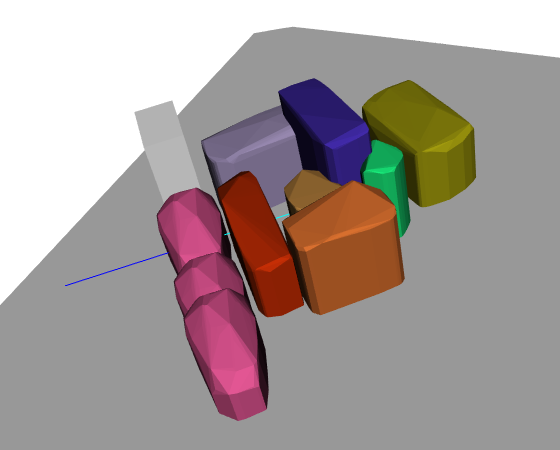
\includegraphics[width=5cm]{Img/block_dir/pushing55.png}
\caption{Evaluating the \ttt{(block\_dir1 * o0)} predicate}\label{fig:block_dir_original}
\end{subfigure}
\caption{Visualization of the computation of \ttt{block\_dir$_i$} predicates. "Evualuating the \ttt{(block\_dir1 * o0)} predicate" means that the algorithm is evaluating for all the objects, except \ttt{o0}, if they collide with \ttt{o0} when pushed along direction 1.}\label{fig:block_dir}
\end{figure}

Considering the kind of objects we are going to interact with, the discrete path  is computed by translating the object along the pushing direction by a length equal to the OBB dimension associated to that direction, until reaching the final pose. Note that no collision detection is done for the object at its initial pose, therefore the total number of poses considered for the pushing path are $n_{poses} = \ceil*{\frac{k \cdot AABB_{dimension}}{AABB_{dimension}}} = \ceil*{k}$, where $k$ is the pushing step defined in Section \ref{subsec:pushing}.

To push an object along a certain direction the robot needs to put its end effector at the opposite side of the object. Therefore object \ttt{o1} can block object {o0} to be moved along a certain direction also in the case the end effector cannot be put in the pushing pose because it would collide with \ttt{o1}. This computation is simply done by transforming the closed gripper mesh model to the pushing pose and check for collision with the other objects, as similarly done for the computation of the \ttt{block\_grasp} predicate.

In Figure \ref{fig:block_dir} is shown graphically the procedure to compute the predicate. 


Note that also the gripper during the pushing action will move, so ideally the collision checking should be done exactly as done for the object. We decided to neglect this and check only for the initial pushing pose in order to relax the planner and not to make it too much conservative. This means that during the pushing action the robot might actually move more than one object. Despite this relaxing strategy the algorithm showed to work fine and cases in which the gripper moved more than one object were really rare.

\begin{algorithm}[h]
\caption{Computation of \texttt{block\_dir} predicates. \\
\textbf{Inputs:} set of objects $O$ (convex hull retrieved with the projection onto the table plane), set of the pushing directions $P_d$ of all the objects, set of the initial pushing pose $P_{poses}$ of all the objects, set of all the pushing paths $P_{path}$ relative to each direction and each object. \\
\textbf{Outputs:} \ttt{block\_dir} predicates}\label{alg:block_dir}
\begin{algorithmic}
\Function{ComputeBlockDirPredicates}{$O$,$P_d$,$P_{poses}$,$P_{path}$}\\
\texttt{block\_dir\_predicates} $\gets$ \textsc{NULL}
\ForAll{$A \in O$}
\ForAll{$d \in P_d(A)$}
\ForAll{$p \in P_{path}(A,d)$}
  \State $A_T \gets$ {\sc transformObject($A,p$)}
\ForAll{$B \in O$}
  \If{$A \neq B$} 
	\State $collision \gets$ \textsc{isThereCollision($A_T$,$B$)}
	\If{collision}
		\State \texttt{block\_dir\_predicates} $\gets$ \textsc{AddPredicate}(\texttt{(block\_dir$_d$ B A)})
	\EndIf
  \EndIf
  \EndFor 
  \EndFor

  \State $closedGripperMesh \gets$ \textsc{trasnformClosedGripperModel}($P_{poses}(A,d)$)
\ForAll{$B \in O$}
\If{$A \neq B$} 
	\State $collision \gets$ \textsc{isThereCollision($closedGripperMesh$,$B$)}
	\If{collision}
		\State \texttt{block\_dir\_predicates} $\gets$ \textsc{AddPredicate}(\texttt{(block\_dir$_d$ B A)})
	\EndIf
  \EndIf
  \EndFor
\EndFor 
\EndFor \\
\Return  \texttt{block\_dir\_predicates}
\EndFunction
\end{algorithmic}
\end{algorithm}  
The computation of this predicate can be appreciated in detail in Algorithm \ref{alg:block_dir}. From that pseudo code can be noted that the complexity of this function to compute the predicate approximatively is %$\mathcal{O}(n \cdot n_{directions} \cdot n_{poses}\cdot (n-1) + (n-1)\cdot n_{directions} )$, 
$\mathcal{O}(n^2)$, where $n$ is the number of objects. 

The computation of this algorithm is the most computational expensive of all the planner since it involves many collision detection phases. In fact the time required to compute this predicate for the example in Figure \ref{fig:block_dir} (considering to push the objects $1.5$ times the OBB dimension relative to the pushing direction) was $\approx 1.115 seconds$, were $\approx 0.869s$ were dedicated to check if the objects would collide when moved, while $\approx 0.239s$ were dedicated to check if the gripper collides with some objects.  

